%\textsl{}%!TEX TS-options = --shell-escape
%!TEX TS-program = pdflatex
\documentclass[%
   10pt,              % Schriftgroesse
   ngerman,           % wird an andere Pakete weitergereicht
   a4paper,           % Seitengroesse
   DIV11,             % Textbereichsgroesse (siehe Koma Skript Dokumentation !)
]{scrartcl}%     Klassen: scrartcl, scrreprt, scrbook, article
% -------------------------------------------------------------------------

\usepackage[utf8]{inputenc} % Font Encoding, benoetigt fuer Umlaute
\usepackage[english]{babel}   % \textsl{}Spracheinstellung

\usepackage[T1]{fontenc} % T1 Schrift Encoding
\usepackage{textcomp}    % Zusatzliche Symbole (Text Companion font extension)
\usepackage{lmodern,dsfont}     % Latin Modern Schrift
\usepackage{dsfont}
%\usepackage{wasysym}
\usepackage{ulem}
\usepackage{graphicx}
\usepackage{eurosym}
%\usepackage{txfonts}
\usepackage{stmaryrd}
\usepackage{amsfonts}
\usepackage{amsmath}
\usepackage{amssymb}
\usepackage{hyperref}
\usepackage{tikz}
\usepackage{multirow}
\usepackage{listings}
\usepackage{etextools}
\usepackage{ifthen}
%\usepackage{TikZ} %phylogenetischer Baum
%\usetikzlibrary{calc, shapes, backgrounds} %für die Phylogenetische bäume
%\usetikzlibrary{automata,arrows}
\usepackage{caption}
\usepackage{units}
\usepackage{subcaption}

% Definition des Headers
\usepackage{geometry}
\geometry{a4paper, top=3cm, left=3cm, right=3cm, bottom=3cm, headsep=0mm, footskip=0mm}
\renewcommand{\baselinestretch}{1.3}\normalsize
\renewcommand{\thesubsection}{\thesection\alph{subsection}}

\def\header#1#2#3#4#5#6#7{\pagestyle{empty}
\noindent
\begin{minipage}[t]{0.6\textwidth}
\begin{flushleft}
\textbf{#4}\\% Fach
#6\\% Semester
Tutor: #2  % Tutor 
\end{flushleft}
\end{minipage}
\begin{minipage}[t]{0.4\textwidth}
\begin{flushright}
\points{#7}% Punktetabelle
\vspace*{0.2cm}
#5%  Names
\end{flushright}
\end{minipage}

\begin{center}
{\Large\textbf{ Blatt #1}} % Blatt

{(Abgabe am #3)} % Abgabedatum
\end{center}
}

\newenvironment{vartab}[1]
{
    \begin{tabular}{ |c@{} *{#1}{c|} } %\hline
}{
    \end{tabular}
}

\newcommand{\myformat}[1]{& #1}

\newcommand{\entry}[1]{
  \edef\result{\csvloop[\myformat]{#1}}
  \result \\ \hline
}

\newcommand{\numbers}[1]{
  \newcounter{ctra}
\setcounter{ctra}{1}
\whiledo {\value{ctra} < #1}%
{%
  \myformat{\thectra}
  \stepcounter{ctra}%
}
\myformat{\thectra}
}
\newcommand{\emptyLine}[1]{
  \newcounter{ctra1}
\setcounter{ctra}{1}
\whiledo {\value{ctra1} < #1}%
{%
  \myformat{\hspace*{0.5cm}}
  \stepcounter{ctra1}%
}
}

\newcommand{\points}[1]{
\newcounter{colmns}
\setcounter{colmns}{#1}
\stepcounter{colmns}
  \begin{vartab}{\thecolmns}
    \numbers{#1} & $\sum$ (7)\\\hline
    \emptyLine{\thecolmns}\\
  \end{vartab}
}

\begin{document}
%\header{Blatt}{Tutor}{Abgabedatum}{Vorlesung}{Bearbeiter}{Semester}{Anzahl Aufgaben}
\header{11}{Alexander Seitz}{1. Februar 2016}{Bioinformatics I}{\\Jonas Ditz \\\& Benjamin Schroeder}{WS 15/16}{3}

\section{Theoretical Assignment - \textit{Coverage statistics}}
\subsection{fraction sequenced}
The used equation is from the script(equation \ref{fraction}.\\	
	\begin{eqnarray}
		f=1-e^{-c} \label{fraction}\\
	\end{eqnarray}
\\	
As a result of using the given coverages $c=1,2,4,8, 14$, table \ref{fractionsTable} is deduced. The last column shows the bases which are not covered when the sequence length is  $L= 248956422 bp$ like in the human chromosome 1.
\\
\begin{tabular}{|c|c|c|c|}
	\hline coverage & fraction covered f & fraction not covered & bases not covered [bp] \\ 
	\hline 1 & 0.63212 & 0.36788 & 91586089 \\ 
	\hline 2 & 0.86466 & 0.13534 & 33693762 \\ 
	\hline 4 & 0.98168 & 0.01832 & 4650882 \\ 
	\hline 8 & 0.99966 & 0.00034 & 84645 \\ 
	\hline 14 & 0.99995 & 0.00005 & 12448 \\ 
	\hline 
	\label{fractionsTable}
\end{tabular} 
\\
The Treponema pallidum chromosome has a length of 1,139,633 bp. If now less than one base can be missed, the not covered fraction is $\leq\frac{1}{1,139,633} =7.16*10^{-6}$. This results in a positive fraction of at least 0.999993.  The coverage is determined with the transformed equation \ref{transformedEquation1} and has a value of 11.87.
\\
\begin{equation}
c=-ln(1-f)
\label{transformedEquation1}
\end{equation}
\\
\subsection{times sequenced}
If there is a coverage of $c=10$, a base has been exactly been sequenced three times with a probability p(3)=0.015 according to the poisson distribution (equation \ref{pois}).
\\
\begin{equation}
p(x)=\frac{c^x}{x!} e^{-c} \label{pois}
\end{equation}
\begin{equation}
p(x)=\frac{10^3}{3!} e^{-10} = 0.015
\end{equation}
The next question was at most three times covered. This can be calculated with equation \ref{poisD}. F(3) has a value of $F(3)=0.018$.

\begin{equation}
	F(n)= \sum_{x=0}^{3} p(x) \label{poisD}	
\end{equation}
\begin{equation}
	F(3)= \frac{10^0}{0!}*e^{-10}+\frac{10^1}{1!}*e^{-10}+\frac{10^2}{2!}*e^{-10}+\frac{10^3}{3!}*e^{-10} = 0.018 \label{poisD}	
\end{equation}
\\
\subsection{}
expected number of gaps
mean contig size
\\
\section{Theoretical Assignment - \textit{Application of the arrival statistic for unitigs}}

The probability whether a unitig is unique can be done with a formula derived from the Lander-Waterman 
model for shotgun sequencing. This formula is
\begin{equation}
 \frac{e^{-c} c^k}{k!}\text{, with } c = \frac{\rho R}{L} \nonumber
\end{equation}
for non-oversampled unitigs and
\begin{equation}
 \frac{e^{-2c} (2c)^k}{k!} \nonumber
\end{equation}
for unitigs that are the result of collapsing two repeats. In these formulas $R$ is the number of reads, $L$ is the length 
of target sequence, $\rho$ is the length of the unitig and $k$ is the number of reads contained by the 
unitig.

In this task we consider a source sequence of length $L = 2Mb$ and $R = 22000$ reads. The length of 
the unitig is $\rho = 3000bp$ and it consists of $k = 100$ reads. With the formulas mentioned above, the 
probability of this specific unitig to be unique is
\begin{equation}
 \frac{e^{-\frac{3000 \cdot 22000}{3000000}} \cdot (\frac{3000 \cdot 22000}{3000000})^{100}}{100!} \approx 5.221 \cdot 10^{-34} \nonumber
\end{equation}
for the case that our unitig is not oversampled and 
\begin{equation}
 \frac{e^{-2\frac{3000 \cdot 22000}{3000000}} \cdot (2\frac{3000 \cdot 22000}{3000000})^{100}}{100!} \approx 1.846 \cdot 10^{-13} \nonumber
\end{equation}
for the case that our unitig is the result of collapsing to repeats.



\section{Theoretical Assignment - \textit{On distances}}
\subsection{}

Consider a tree $T$ constructed with $D$ and the four nodes $i,j,k,l \in T$. Since $D$ is ultrametric, 
the following four inequalities have to hold:
\begin{align}
 d(i,j) &\le max \left\lbrace d(i,k), d(j,k) \right\rbrace \nonumber \\
 d(i,j) &\le max \left\lbrace d(i,l), d(j,l) \right\rbrace \nonumber \\
 d(k,l) &\le max \left\lbrace d(i,k), d(i,l) \right\rbrace \nonumber \\
 d(k,l) &\le max \left\lbrace d(j,k), d(j,l) \right\rbrace \nonumber
\end{align}
W.l.o.g we can assume that $d(i,k) = d(j,k) = d(i,l) = d(j,l)$. With that assumption we can rewrite 
the inequalities as
\begin{align}
 d(i,j) + d(i,j) &\le d(i,k) + d(j,l) \nonumber \\
 d(k,l) + d(k,l) &\le d(i,l) + d(j,k) \nonumber
\end{align}
And also the following inequality is valid:
\begin{equation}
 d(i,j) + d(k,l) \le max \left\lbrace d(i,k) + d(j,l), d(i,l) + d(j,k) \right\rbrace \nonumber
\end{equation}
As one can see, that is the Four-Point-Condition (4PC) and a metric fulfill 4PC if and only if it is 
additive. So $D$ is a tree metric $\square$

To show the back direction one consider the four elements $A, B, C, D \in X$ of a taxa $X$ and the 
following distance matrix:
\begin{equation}
 D = \begin{bmatrix}
        & B & C & D \\
      A & 7 & 6 & 5 \\
      B &   & 3 & 6 \\
      C &   &   & 5
     \end{bmatrix} \nonumber
\end{equation}
One can see in the script of this lecture that $D$ is a tree metric. But the Three-Point-Condition 
(3PC) is not fulfilled as can be easily shown. To fulfill 3PC the following inequality has to be 
valid:
\begin{equation}
 d(A,B) \le max \left\lbrace d(A,C), d(B,C) \right\rbrace \nonumber
\end{equation}
but
\begin{equation}
 7 \nleq max \left\lbrace 6, 3  \right\rbrace \nonumber
\end{equation}
So $D$ does not fulfill 3PC and thus $D$ is not ultra metric. $\square$

\subsection{}

\begin{figure}[t]
 \centering
 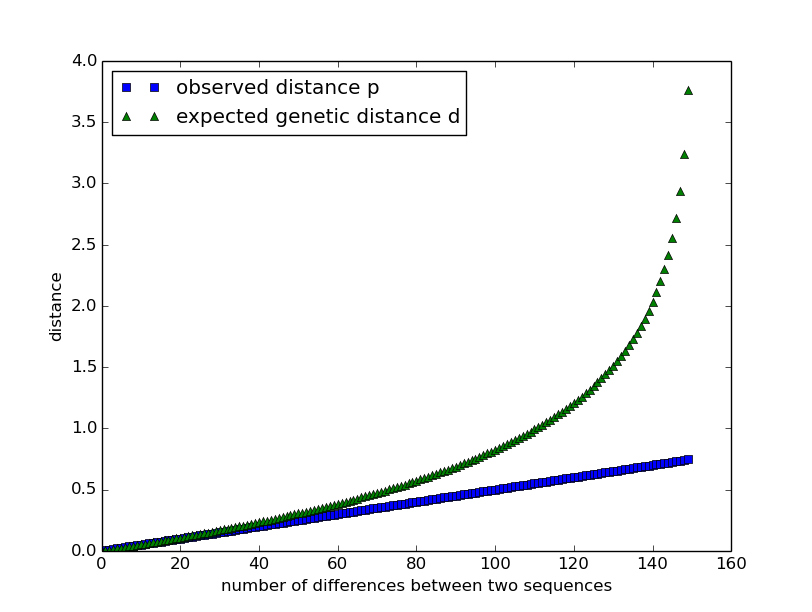
\includegraphics[width=0.6\textwidth]{exec3bFigure.png}
 \caption{Behavior of observed distance $p$ and expected genetic distance $d$ of two non-saturated sequences. Both sequences are of length 200.}
 \label{fig:pdRelationship}
\end{figure}

There are different methods to estimate the (evolutionary) distance between two sequences. The easiest 
one is to simply calculate the Hamming distance. This is called the observed or $p$-distance. $p$-distance 
is just suitable for closely related species, since it is not able to detect superimposed mutations, i.e. 
mutations that happened at a position that was already mutated, previously. A correction for observed 
distance was formulated by Jukes and Cantor. The Jukes-Cantor transformation corrects the $p$-distance 
to take, among others, superimposed events into account. This correct distance is called the expected 
genetic distance $d$. An important note is that JC transformation does 
not work for sequences that are saturated w.r.t. each other. So Figure \ref{fig:pdRelationship} shows 
the relationship between $d$ and $p$ for non-saturated sequences of length 200. As one can see the 
observed distance $p$ is constantly underestimating the genetic distance for more distant sequences. 
Especially, if both sequences are close to be saturated, the difference between $d$ and $p$ shows 
that $p$ cannot give a reliable result. So for sequences/species that are evolutionary close to each 
other both measurements $d$ and $p$ give almost the same result. But the further away the last common 
ancestor of both sequences the larger is the difference between observed distance and expected genetic 
distance. 

%\begin{thebibliography}{20}
%	
%\end{thebibliography}


\end{document}